\section{Experiment Design}\label{sec:experimentdesign}

\begin{figure}[t]
\begin{subfigure}[t]{0.58\textwidth}
    \centering
    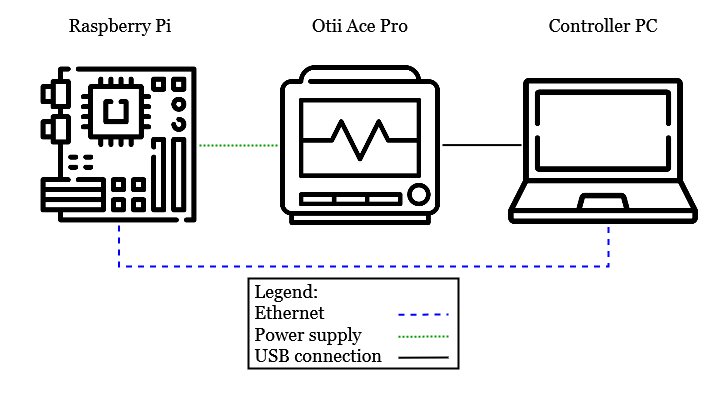
\includegraphics[width=\textwidth]{images/experiment.png}
    \caption{Experiment design for measuring power draw and runtime of \gls{sut} while executing \gls{pyperformance} benchmarks.}
    \label{fig:design}
\end{subfigure}
\hspace{\fill}
\begin{subfigure}[t]{0.4\textwidth}
    \centering
    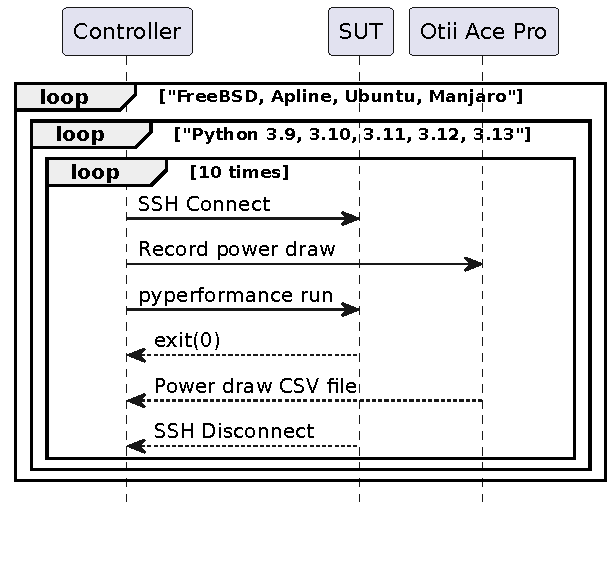
\includegraphics[width=\textwidth]{images/scenario.pdf}
    \caption{Interactions between the controller computer initiating power draw recordings and benchmark executions.}
    \label{fig:sequence}
\end{subfigure}
\caption{Illustration of our experiment design.}\label{fig:exp_scen}
\end{figure}





\autoref{fig:design} illustrates our experiment design.
The \toolname{Otii Arc Pro} in the center, powers a \toolname{Raspberry Pi} (\gls{sut}) via USB-C.
At the same time, it serves as a power meter recording the power draw of the \gls{sut} (illustrated by a green line).
A controller computer (to the right in \autoref{fig:design}) is connected via USB to the power meter (black line).
Using the \toolname{Otii 3 Desktop App}
% https://docs.qoitech.com/user-manual/otii/software/otii3-desktop-app
and the \toolname{Otii Automation Toolbox}
% https://www.qoitech.com/automation-toolbox/
, the controller computer can trigger a measurement and collect all power meter recordings automatically.

Both the \gls{sut} and the controller computer are connected via ethernet to a local network (blue line).
By that connection, the controller computer initiates executions of \acrlong{pyperformance} on the \gls{sut}.

Not illustrated in \autoref{fig:design} is a 25V lab power supply powering the \toolname{Otii Arc Pro} and a room fan that is placed next to the \gls{sut} to keep \gls{cpu} temperature on a constant level.

Prior to the experiment, we prepare four SD-cards.
One with \projname{FreeBSD}, \projname{Alpine}, \projname{Manjaro}, and \projname{Ubuntu} Linux respectively\todo{Add precise versions+kernel and libc versions}, see our replication kit for details.
On each of these, we automatically install the five versions of \python (\cpv{9} to \cpv{13}) from source together with the \gls{pyperformance} tool.\todo{Did that include tuning? OB: No, but maybe it should?}
Each operating system and each version of \python is setup in default configuration.



% A large fan is set up to continually cool the RPi, and CPU temperature is then queried directly on the RPi through another SSH terminal on the PC, before, during, and after benchmarks.
% This is to make sure that rising CPU temperature doesn't skew the measurements for longer benchmarks, since CPUs are known to perform worse at higher temperatures\cite{benoit2020impact}.
% TODO: Move that to Threats
% Throughout the entire benchmarking process, the CPU temperature never rises above 37$^{\circ}$C, which is deemed satisfactory for consistency of results.
% OSs are installed in their default configurations to make sure that any potential differences in energy consumption between them can be explained by the OS implementation specifics alone, and not by the quality of performance optimizations made by the user.

Per configuration of \gls{cpu}, \gls{os}, and version of \python, we execute the \gls{pyperformance} benchmarks ten times\todo{@oskar: you experiment script does it 11 times, why? OB: An artefact, in case one of them failed. Could be changed as it no longer serves a purpose.} and record power draw for each invocation of the benchmarks, see the inner most loop in\autoref{fig:sequence}.
Note, per default, \gls{pyperformance} executes each benchmark 20 times per invocation of the tool.
We omit to illustrate this internal behavior in \autoref{fig:sequence} and consider \gls{pyperformance} as a black box in our experiment.
The ten invocations of the \gls{pyperformance} benchmarks is repeated five times, i.e., on each version of \python (\cpv{9} to \cpv{13}), see nested loop on level two in \autoref{fig:sequence}.
These two steps of the experiment are automated via scripts.
The benchmarks are invoked 10 times per version of \python on each of the four \gls{os}, \projname{FreeBSD}, \projname{Alpine}, \projname{Manjaro}, and \projname{Ubuntu} Linux, see outer most loop in \autoref{fig:sequence}, and in turn on each of the two \gls{sut} \toolname{Raspberry Pi 3B+} and \toolname{4B} respectively.
These latter two experiment steps are manual since they require to power-down the respective \gls{sut} and replace the SD-card or to replace the \gls{sut} (not illustrated in \autoref{fig:sequence}).

In total, we collect 400 measurements, i.e., 10 invocations of \gls{pyperformance} on five versions of \python on four \gls{os} on two \gls{sut}.
All collected measurements are automatically stored in CSV files, which we aggregate for further analysis for the following sections.